\documentclass{article}
\usepackage[fleqn]{amsmath}
\usepackage{bm}
\usepackage{graphicx} % Required for inserting images
\usepackage[legalpaper, portrait, margin=1in]{geometry}
\usepackage[l3]{csvsimple}
\usepackage[section]{placeins}
\usepackage{float}

%command to add S to the figure ids
\renewcommand{\thefigure}{S\arabic{figure}}
%command to add s to the table ids
\renewcommand{\thetable}{S\arabic{table}}


\title{Supplement}
\date{}
\begin{document}

\maketitle
\listoffigures
\listoftables
\section{Drought Survival Model}


There are three submodels to the full drought survival model. The survival model, the size model, and a prior model, which are fit simultaneously. Unless noted, the Normal distribution is parameterized in terms of the mean and standard deviation.

The log-odds of survival are modeled as a function of relative growth rate (\(RGR\)) and size (\(Size\)) at the beginning of the terminal drought trial:
\begin{align*} 
&s_i \sim Bernoulli(p_i) \\
&logit(p_i) = \alpha + \beta_{rgr} \times RGR^*_i + \beta_{size} \times Size^*_{i,tmax}
\end{align*}

The index \(i\) indicates the individual and the index \(t\) is the time point when size was measured. (\(tmax\) is the time at the beginning of the drought trial). Asterisks (e.g. \(RGR^*\)) indicate that the variable has been standardized to have a mean of 0 and standard deviation of 1. In this portion of the model \(\alpha\) is the expected log-odds of survival of an individual with mean \(Size\) and \(RGR\). The coefficients, \(\beta_{.}\), are the change in log-odds of survival for a single standard deviation change in the variable of interest.

The model for size is an exponential growth model where size at a given time point is an exponential function of original size, growth rate, and age: \(size_t = size_0e^{rgr*age}\). The log of size was taken so that the submodel model can be expressed as:

\begin{align*}
&\log(Size_{i,t}) \sim Normal(\mu_{i,t},\space \sigma) \\
&\mu_{i,t} = \log(Size_{i,0}) + RGR_i \times Age_{i,t} \\
&\log(Size_{i,0}) = \gamma + \beta_{seed}\times SeedSize^*_i + \eta_i
\end{align*}

Where the initial seedling size is modeled as a function of seed size where \(\log(Size_.0)\) increases by \(\beta_{seed}\) with an increase of one standard deviation of seed size and has an expected value of \(\gamma\) at the mean seed size. An error term \(\eta\) is added and is allowed to correlate with \(RGR\), which is the change in \(\log(Size)\) in one day.

Finally, a prior model specifies prior distributions for all unknown variables in the submodels above.

\begin{align*}
&\begin{bmatrix}
RGR_i \\
Age_{i,tmax} \\
SeedSize_i \\
\eta_i
\end{bmatrix} = MVNormal \left( \begin{bmatrix}
\mu_{rgr} \\
\mu_{age} \\
\mu_{seed} \\
0
\end{bmatrix}, \space diag(\bm{\tau})\space  \mathbf{R}\space diag(\bm{\tau}) \right) \\
&\mathbf{R} \sim LkjCorr(2) \\
&\tau_. \sim Exponential(1) \\
&\mu_{rgr} \sim Normal^+(0, 1) \\
&\mu_{age} \sim Normal^{0-14}(14, 4) \\
&\mu_{seed} \sim Normal(0, 1) \\
&\beta_., \alpha, \gamma \sim Normal(0, 1) \\
&\sigma \sim Exponential(1)
\end{align*}

Where \(\mathbf{R}\) is a correlation matrix and the \(LkjCorr(\theta)\) distribution is a distribution over correlation matrices where \(\theta\) controls the strength of expected correlations. A \(\theta\) of 1 gives equally likelihood to all correlation matrices. A \(\theta\) of 2, as used here, is weakly regularizing toward weak correlations (95\% of the probability for the correlations falls between ~ -0.7 and 0.7. \(\bm{\tau}\) is a vector of standard deviations with \(diag(\bm{\tau})\) being a diagonal matrix with the elements of \(\bm{\tau}\) on the diagonal and 0's elsewhere. Subscripts over distributions indicate truncation (e.g. \(Normal^+\) indicates a normal distribution truncated to positive values). 

\section{Selection Gradients}

The linear selection gradient can be estimated as \(\frac{Cov(w, z)_T}{\sigma^2_z}\). Where the subscript \(T\) indicates the covariance between relative fitness (fitness scaled so that it has a mean of 1) and the trait that is traceable back to the trait excluding paths through correlations to other traits. Typically this is achieved through multiple regression, but for more complex models, this covariance can be isolated using path analysis. Figure \ref{fig:path_model} shows the path model evaluated in this paper. Given this model \(Cov(\omega,\space RGR) = \sigma_{rgr}\sigma_{\omega}(h + ag + dbg + fcg)\). The covariance that is due to directed paths from \(RGR\) to \(\omega\) is \(\sigma_{rgr}\sigma_{\omega}(h + ag)\) and so the selection gradient for relative growth rate is: \(\frac{\sigma_{rgr}\sigma_{\omega}(h + ag)}{\sigma^2_{rgr}}\). Multiplying this by \(\frac{\sigma_{rgr}}{\sigma_{\omega}}\) yields the standardized regression gradient which is \(h + ag\).

\section{Validating computation and model fit}

\section{Figures}

\begin{figure}[!htb]
    \centering
    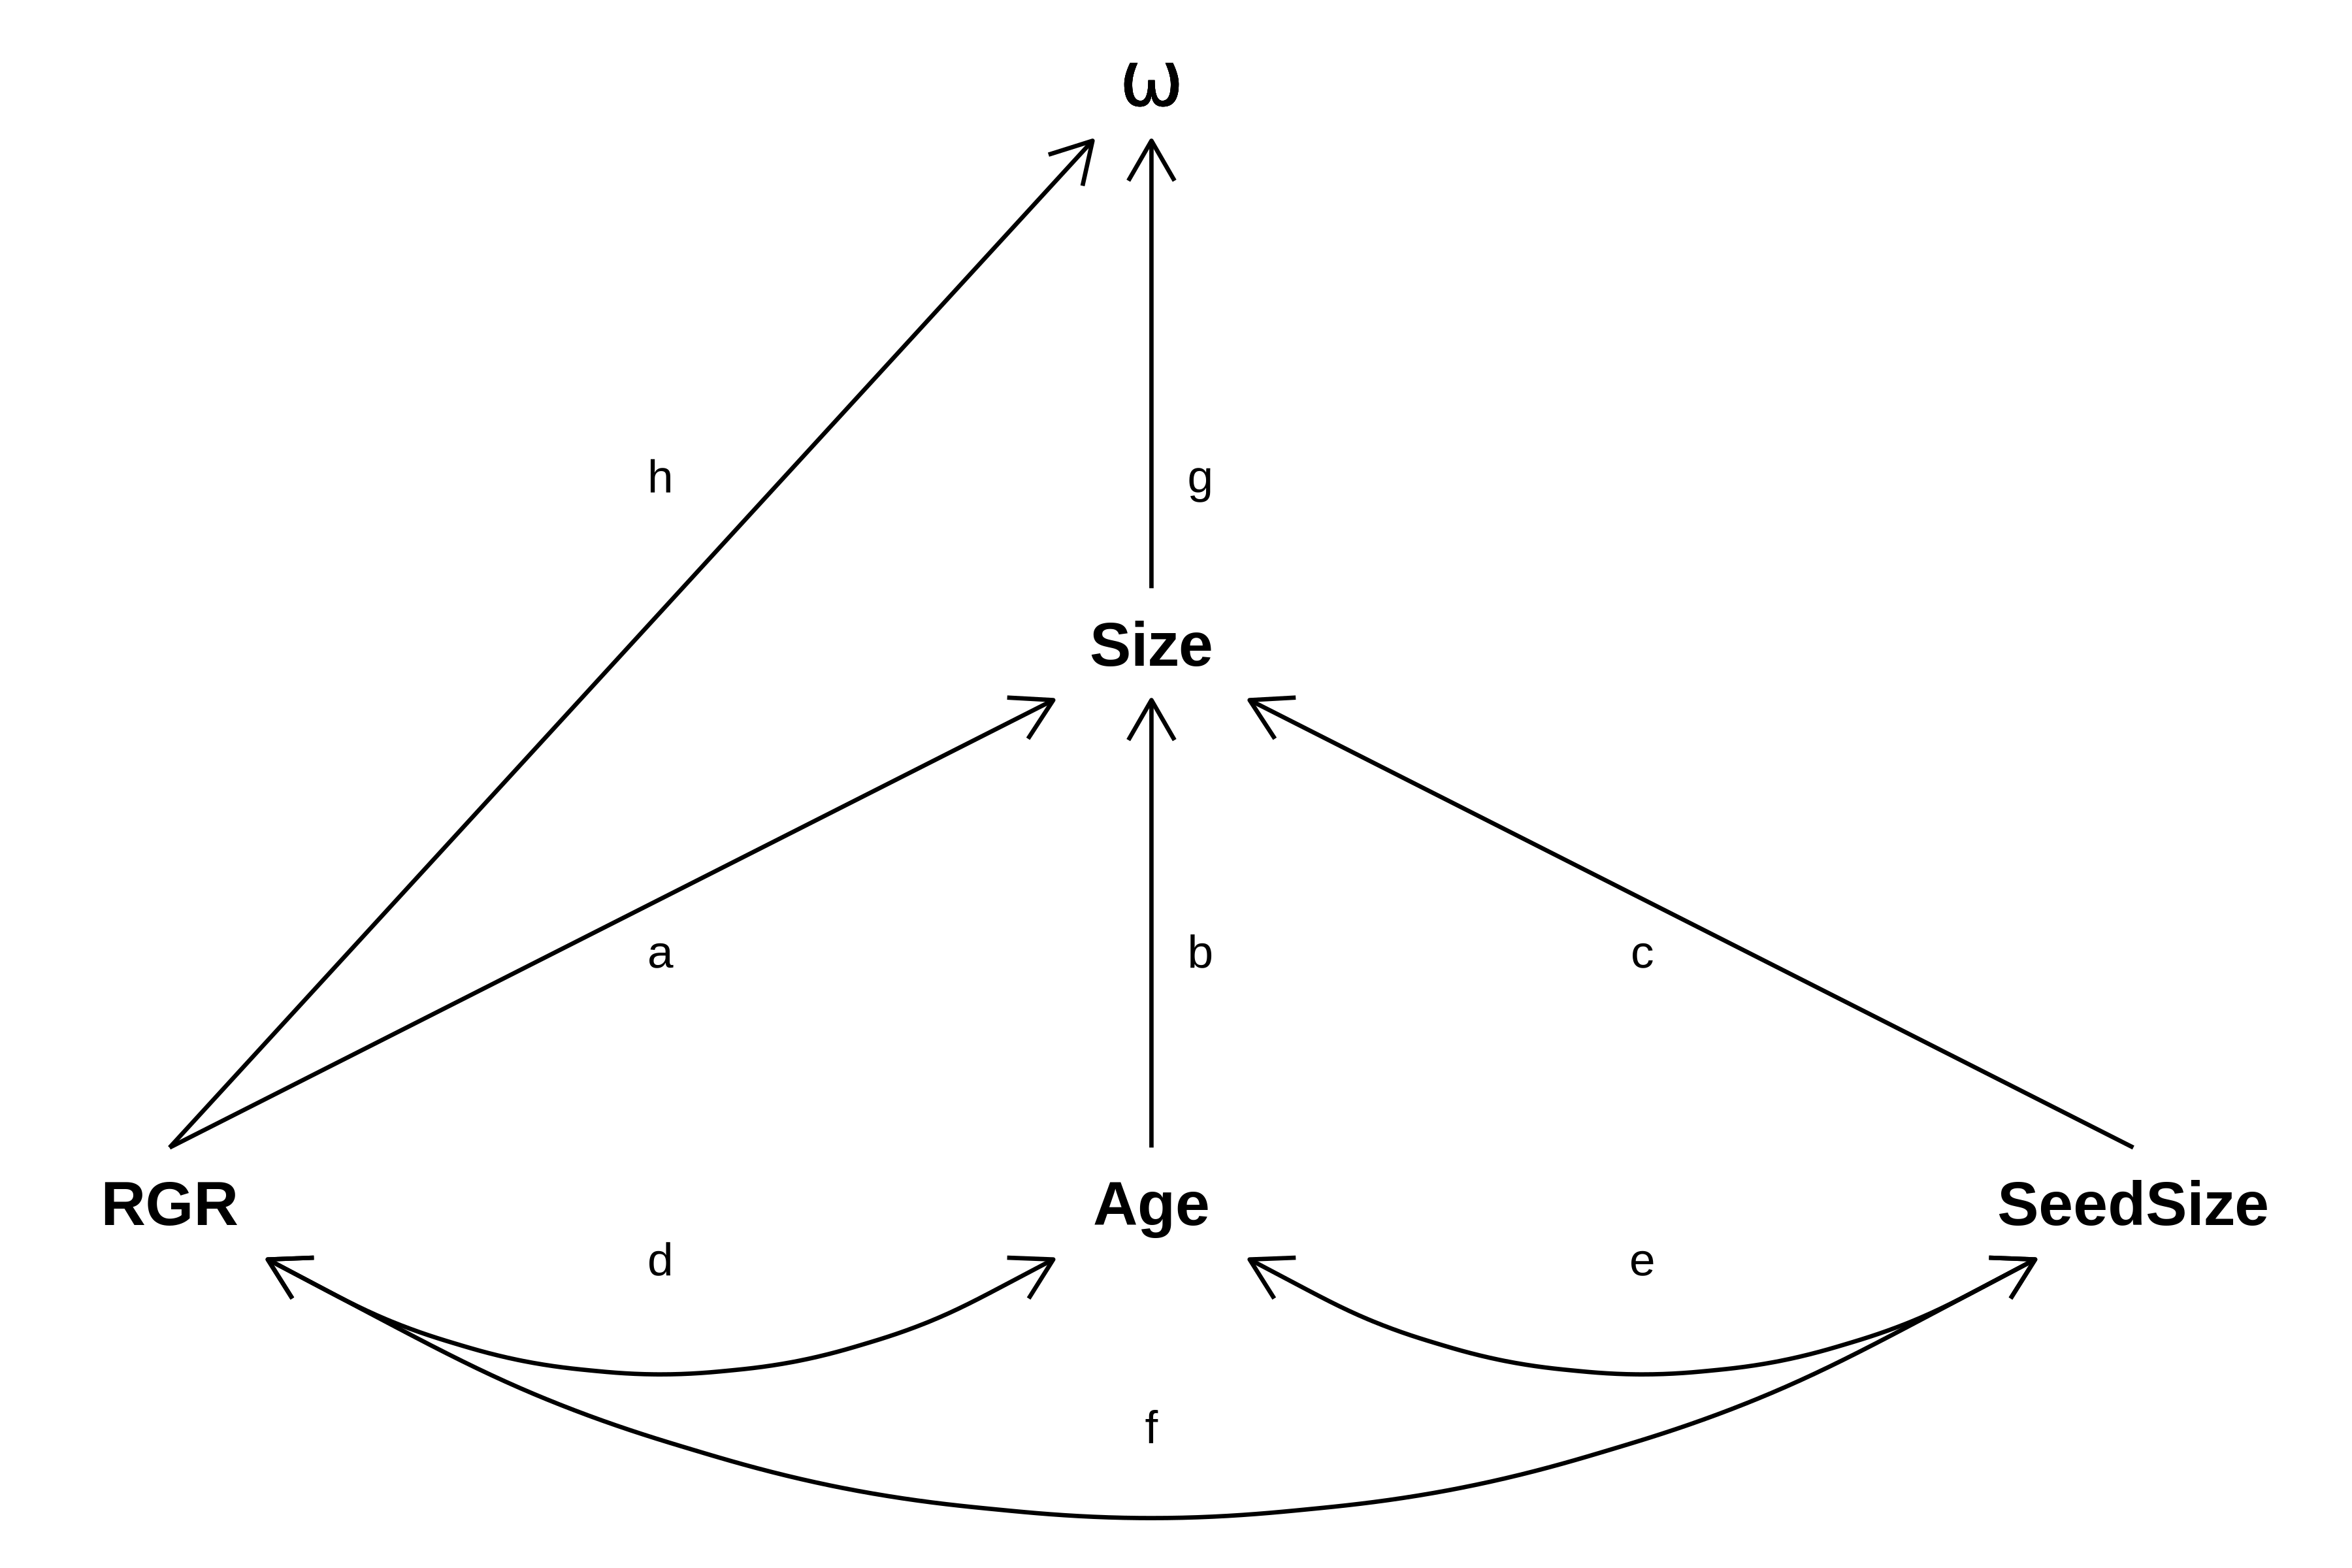
\includegraphics[width=1\linewidth]{plots/path_model.png}
    \caption{Path model relating traits to fitness}
    \label{fig:path_model}
\end{figure}

\section{Tables}

Table \ref{tab:means} shows the posterior for estimates of the trait mean for each cross. \(\Delta/E(F_2)\) is the deviation from the additive/dominance expectation scaled by the expected \(F_2\). Columns indicate the line, posterior percentiles, and posterior mean.

\begin{table}[H]
    \centering
    \begin{tabular}{|c|c|c|c|c|c|c|c|}
         \hline Line  & 2.5\% & 25\% & Mean & 75\% & 97.5\% & Trait \\ \hline
        \csvreader[late after line = \\\hline]{posteriors/traits.csv}{}{
        \csvcoli & \csvcolii & \csvcoliii & \csvcoliv & \csvcolv & \csvcolvi &  \csvcolviii
        }
    \end{tabular}
    \caption{Posteriors for trait means}
    \label{tab:means}
\end{table}

Table \ref{tab:mean_diffs} shows the posterior for trait mean differences between lines. The comparison column indicates the two lines being compared (e.g. LON-CAL is the posterior for the longiflorus trait mean minus the calycinus trait mean). Posterior percentiles and mean are indicated as well as the proportion of the posterior that is less than 0.

\begin{table}[H]
    \centering
    \begin{tabular}{|c|c|c|c|c|c|c|c|}
    \hline Trait & Comparison & 2.5\% & 25\% & Mean & 75\% & 97.5\% & Prop. \textless  0 \\ \hline
        \csvreader[late after line = \\\hline]{posteriors/diffs.csv}{}{
        \csvcoli & \csvcolii & \csvcoliii & \csvcoliv & \csvcolv & \csvcolvi & \csvcolvii & \csvcolviii
        }
    \end{tabular}
    \caption{Posteriors for trait mean differences between lines.}
    \label{tab:mean_diffs}
\end{table}

Table \ref{tab:survival_coefs} summarizes the posterior distributions for the effects of \(RGR\) and \(Size\) on the log-odds of survival. The posterior percentiles and mean are shown as well as the proportion of the posterior that is greater than 0.

\begin{table}[H]
\centering
\begin{tabular}{|c|c|c|c|c|c|c|}
 \hline Coefficient & 2.5\% & 25\% & Mean & 75\% & 97.5\% & Prop. \textgreater  0 \\ \hline
\csvreader[late after line = \\ \hline]{posteriors/betas.csv}{}{
\csvcoli & \csvcolii & \csvcoliii & \csvcoliv & \csvcolv & \csvcolvi & \csvcolvii
}
\end{tabular}
\caption{Posteriors for the survival submodel coefficients}
\label{tab:survival_coefs}
\end{table}

Table \ref{tab:path_coefs} summarizes the posterior for the path coefficients (a,b,c,g,h) and correlations (e,f,g). It also summarizes the posteriors for the standardized selection gradients (\(\beta_.\). Posterior percentiles, means, and proportion greater than 0 are provided. 

\begin{table}[H]
\centering
\begin{tabular}{|c|c|c|c|c|c|c|}
 \hline Path & 2.5\% & 25\% & Mean & 75\% & 97.5\% & Prop. \textgreater  0 \\ \hline
\csvreader[late after line = \\ \hline]{posteriors/corrs.csv}{}{
\csvcoli & \csvcolii & \csvcoliii & \csvcoliv & \csvcolv & \csvcolvi & \csvcolvii
}
\end{tabular}
\caption{Posteriors for correlations and path coefficients}
\label{tab:path_coefs}
\end{table}

\end{document}
